\documentclass [10pt,fleqn,a4paper]{jsarticlek}
\usepackage[dvipdfmx]{graphicx,color}
\usepackage[deluxe]{otf}
\usepackage{amsmath,ceo,daisu}

\begin{document}
作図の仕方について，例を使って説明します．図を作るソフトはMathematicaまたは
WinTpic（Windows版のみ）です．図をラフに描いたらAdobe Illustratorで加工します．2次元のグラフまでなら，WinTpicで描けますが，3次元は不可能です．
\begin{Mgwaku}(4,10)[\textgt{〈この問題の解答を完成せよ〉}]
\begin{reidai}
\lineskip=4pt
\lineskiplimit=4pt
$xy$平面上の2曲線$C_1:y=x^2,\;C_2:y=2^x$について次の問に答えよ．ただし自然対数について$\dfrac{11}{16}<\log 2<\dfrac{7}{10},\;\dfrac{8}{5}<\log 5<\dfrac{13}{8}$であることは証明せずに用いてよい．

\begin{shomonr}
2曲線の交点の1つは$-\dfrac{4}{5}<x<-\dfrac{1}{2}$にあることを示せ．
\end{shomonr}

\begin{shomonr}
2曲線はいくつの部分を囲むか．また，このうちで，面積が一番小さい領域の面積を求めよ．なお，2曲線$y=f(x),\;y=g(x)$が囲む領域とは，
\[
f(a)=g(a),\;f(b)=g(b),\;f(x)<y<g(x)\;\;(a<x<b)
\]
のように表される領域をいう．
\syutten[3000,東大・理科（第1問）]
\end{shomonr}
\end{reidai}

\end{Mgwaku}
\lineskip=4pt
\lineskiplimit=4pt
【{\gt Mathematicaの場合}】まず，Mathematicaでグラフを描きます．Mathematicaを起動し，グラフを描画するコマンドを書き込みます．例えば
\begin{verbatim}
g=Plot[{2^x, x^2},{x,-5,5},PlotPoints -> 100,
PlotRange -> {{-3,5},{-1,20}},AspectRatio -> Automatic,
Ticks -> None]
\end{verbatim}

オプションでPlotPointsは100，AspectRatioはAutomatic，TicksはNoneに設定してください．区間を100分割して線分で結んで曲線を描きます．縦横の比を正確にするときはAutomaticにして，適宜変更します．今の場合，縦に長すぎるので，AspectRatio$->$1にすると，下図を描きます．矢印はマイナスと不等号で打ち込むと自動で変換します．Ticksは常時Noneにしてください．軸目盛り付けなしです．EnterキーまたはShift + Enterでグラフが表示されます．これはキーボードによって違います．グラフがうまく表示できたらMathematicaのファイルを保存します．2014-東大-1.nbのように，日本語で名前を付けることができます．\\
次にepsファイルの書き出しをします．方法は2つありますが，Mac版のMathematicaのversion9はどちらの方法でもうまくいかないという，呆れたバグがあります．バグレポートを出してあり，Wolframも確認していますが，いまだにバグフィックス版を出していません．世界で一番よく使っている私をないがしろにするから，こんなバグも発見できないのです．きっと，次のversionでバグフィックスをして，しらばっくれるつもりです．Windows版はバージョンアップをしていないので，どうなっているか，不明です．Mac版の場合は，version7以前で行ってください．表示されたグラフをマウスでコチッと選択し，メニューから，ファイル〜選択範囲の形式保存を選び，フォーマットをepsにして，名前を適当につけて，保存ボタンを押します．もう1つの方法は，\\
Export[FileNameJoin[{NotebookDirectory[], "g.eps"}], g]
\\
でexportする方法です．ver7は，この方法はバグだそうです．ですからver7以前で，「選択範囲の形式保存」で行ってください．

Windows版のバージョン8でも試してもらいましたが，どうも，同様に駄目なようです．

\h【WinTpicの場合】安田は詳しくは知りません．

\h【{\gt Adobe Illustratorで加工}】まず，同梱の「安田フォント」をフォントフォルダに入れてください．\\
Macの場合は，ユーザフォルダ（パソコン所有者の名前がついたフォルダ）の中のライブラリを表示（最新のOSでは標準では表示されない．ユーザフォルダ内で，optionキーを押すとメニューの移動欄に表示される．あるいはメニューの「フォルダへ移動」で/Libraryまたは/ライブラリを入れてリターンキーを押す）し，入れます．\\
Windowsの場合は\\
CドライブのWindowsフォルダ内のFontsフォルダを開いて，Ceol-Bold.ttfなどの，拡張子ttfがついているフォントファイルをFontsフォルダに入れます．CeoPCTrueフォルダを入れるのではなく，その中身を入れます．\\

Macの場合，IllustratorのアイコンをDock（ソフトのアイコンが一列に並んでいる場所）の上に出しておきます．Windowsの場合なら，Illustratorのショートカットを自動で作ってくれればよいし，自動で作ってくれないなら，自分で作っておきます．Windowsの「ショートカット」という用語には違和感を感じます．勝手な用語を作るのはやめるべきだと思いますね．これはやはりエイリアスと，ちゃんとした業界用語を使うべきだろうと思います．\\
同梱のイラストレータのファイルzukeimoto.epsをコピーして，名前を適宜変えておきます．その場所で複製するのは，アイコンをつかんで，optionキーを押しながらどこかに移動します．ファイル名を変えるときには，ファイル名のところにマウスのポインタを置いて，名前が選択されれば変えられるし，そうでなければ，リターンキーを押すと，名前が選択できます．今はgraf-1.epsとします．\\
さきほどのグラフg.epsを，DockのIllustratorのアイコン上に落として開きます．図の本体をコピーしてきてgraf-1.epsに貼り付けます．\\
\H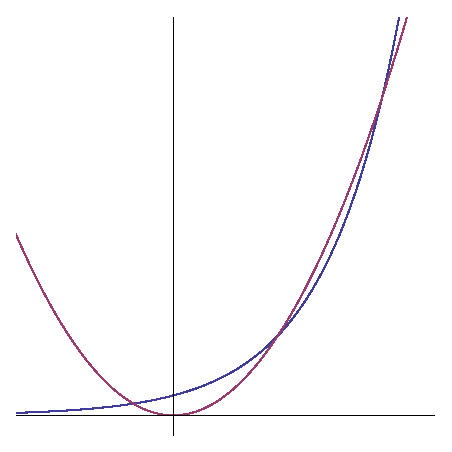
\includegraphics[width=3.5cm]{g.eps} \\
このままではいろいろな意味で使えません．今回の書籍は白黒（グレースケール）でないといけません．
画面の左下方に四角い枠があるので，その枠内に収まるようグラフを移動・縮小します．この枠はTeXへ取り込んだとき標準で4.5cm四方の出力になるようとってあります．枠内の直交する2直線は不要であれば削除してください．Mathematicaから引き連れてきたグラフの囲み枠もいずれは削除しますが，当初は残しておきます．下でパスファインダーを掛けるとき，これがないと，うまく分割されないからです．

図形を調整して行きます．メニューバーのウィンドウから線，カラー，パスファインダー，レイヤー，CADtoolなど必要なツールを指定して画面上に出しておきましょう．一番大きなツールパレットに，矢印の選択ツールがあります．黒い選択ツールは，グループ化された全体を選択し，白い矢印（ダイレクト選択ツール）は部分を選択します．黒い選択ツールで，さきほど貼り付けたグラフ全体を選択指定し，メニューの「編集〜カラーを編集〜グレースケールに変換」します．色のついたものをグレースケールに変換すると，黒線になりません．線を幅0.8pt，色K100％に設定します．線は曲線も直線も座標軸も一律にこの設定でけっこうです．太線にするときには，ハサミツールで切り，ダイレクト選択ツールで選んでから，線幅を1.5ptにします．

図形で塗り潰す部分があるときは，最初の図形全体の枠線がその部分の複製を作って網掛けをし，重ね合わせます．まず，この複製をします．複製するときはoptionキーを押しながら，横へ移動して離します．複製したものを全体選択して，パスファインダーの分割を適用します．図形には「塗り」と「線」があります．塗りをK20％，線幅を0.8ptに設定します．これで複製の図に網掛けが施されました．図に不要な部分があるのが普通です．それをれダイレクト選択ツールで削除します．この網掛けした図を移動して元の図に重ね合わせ，再背面へ配置します．重ね順はメニューバーのオブジェクトから指定できます．これで塗り潰しが完成です．塗り潰し処理がすべて完了したら，レイヤーメニューで「すべてのレイヤーを結合」に固定します．

座標軸の先端に矢印をつけます．矢印の付け方は，Illustratorのversionによって違います．CS6なら，線のパレット内にあります．矢印のどちら側につけるかを考え，矢印の種類は「矢印2」，線幅0.8ptの場合，倍率は65％にします．CS5ならメニューの「効果〜スタイラズ〜矢印をつける」です．CS4,CS5ならばイラストレータのプラグインで，矢印の形を変えたり，垂直マークを付け加えたものyasudayajirusiCS4があります．CS4,CS5のイラストレータのプラグイン〜Illustrator フィルタ内に入れます．CS6用は完成していません．

メニューのその他，曲線の長さ等，微調整してください．必要に応じて垂線や補助線を入れます．主要な線の線幅は0.8pt，引き出し線など補助的な線は0.5pt，色は必ずK100％です．必要に応じて，破線にチェックを入れ，線分4pt，間隔1.8ptに指定します．図中に文字や式を付加します．画面上に整形済みの文字や記号が用意されているので，必要なものをそのまま移動して，あるいは別の文字に編集するなどして利用してください．フォントは斜体がceolItalic，立体がceol Regular，ギリシア文字がCeo Symbol，サイズは基本的に10pt，指数は6ptです．数式が座標軸などの図形要素に重なって見づらい場合は，白塗りの長方形を作って数式の下に挟みます．つまり図形の上に白塗り長方形，その上に数式と重ねます．また，図形と数式をつなぐヒキダシ罫を入れる場合は，CAD円弧ツールを使って線幅0.5pt，塗りなしの曲線を描きます．図の調整がすべて終わったら，周囲の4.5cm枠を透明に変更します．最後に図全体を選択指定し，オブジェクトのグループ設定をします．ファイルを上書き保存します．このあと文字のアウトラインをとりますが，アウトラインをとったあとは文字の修正ができなくなってしまいますので，必ずこの時点でアウトラインを取らないファイル（変更が出た場合のために）ファイルを保存しておきます．現時点では下記のようです．

\H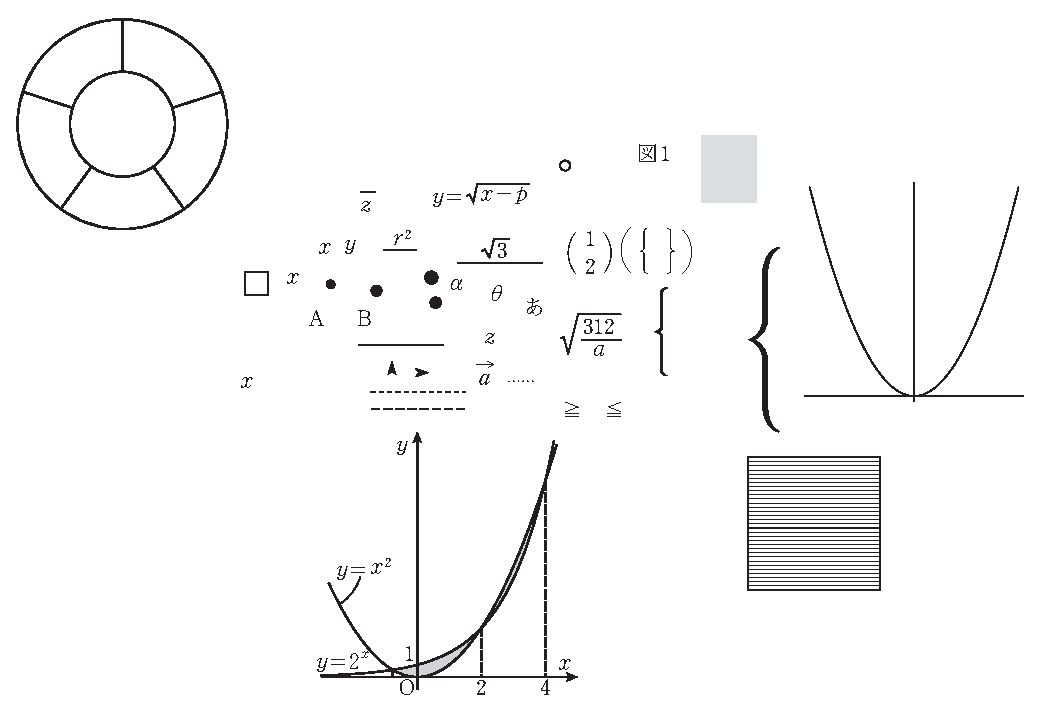
\includegraphics[width=5cm]{zu-1.eps} 

Command + Aで全選択し，メニューバーの書式から「アウトラインを作成」を選びます．あるいはコマンド+A，コマンド+shift+Oとします．文字を図形に変換するのです．それをしないと，文字化けが起こります．画面上のいらない図形要素は削除します．消し残しがないかCommand + Aで確認します．またカラーが掛かっていないか，確認してください．Command + Aで全選択し「編集〜カラーを編集〜グレースケールに変換」します．これで完成です．ファイルを別名で保存します．eps形式，バージョンはCS5です．今は2014-toudai-ri-1-1.epsにしました．慣れると下の図は1枚で20分くらいです．\\
\H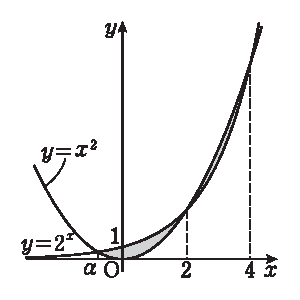
\includegraphics[width=3.5cm]{kari-2014-toudai-ri-1-1.eps} 

空間の曲面は下のように描きます．今は平面に緑色をつけてみました．
\begin{verbatim}
Q[s_] := {s, 1 - s, 2 s - 1};
U[t_] := {{Cos[t], -Sin[t], 0}, {Sin[t], Cos[t], 0}, {0, 0, 1}};
g1 = ParametricPlot3D[Evaluate[U[t].Q[s]], {s, 0, 1}, {t, 0, 2 Pi}, 
  Axes -> None, Boxed -> False, ViewPoint -> {2, -1, 0.8}];
g = Show[g1, 
  Graphics3D[{Green, 
    Polygon[{{1, -1, 1}, {1, 1, 1}, {-1, 1, -1}, {-1, -1, -1}}]}],
  PlotRange -> {{-1.5, 1.5}, {-1.5, 1.5}, {-1.5, 1.5}}, 
  SphericalRegion-> True,
  Boxed -> False]
\end{verbatim}

\includegraphics[width=3.5cm]{2004-keiou-ri-5.eps}

\end{document}